\documentclass{article}
\usepackage{geometry}
\usepackage{graphicx}
\newgeometry{margin=0.5cm}

\title{Mosquito species this summer}
\usepackage{Sweave}
\begin{document}
\Sconcordance{concordance:mosq29octtype.tex:mosq29octtype.Rnw:%
1 6 1 1 0 2 1 1 7 4 1 1 28 1 2 41 1}


\begin{center}
\subsection*{What kind of mosquitos were most prevalent this summer?}
\end{center}
The detection of Aedes albopictus mosquitoes (which are capable of carrying Dengue) prompted a more general conversation about which mosquito genus/species were most prevalent this summer, and which accounted for the early August and mid-September spikes.  What follows are graphical and tabular overviews of that information.
\begin{center}
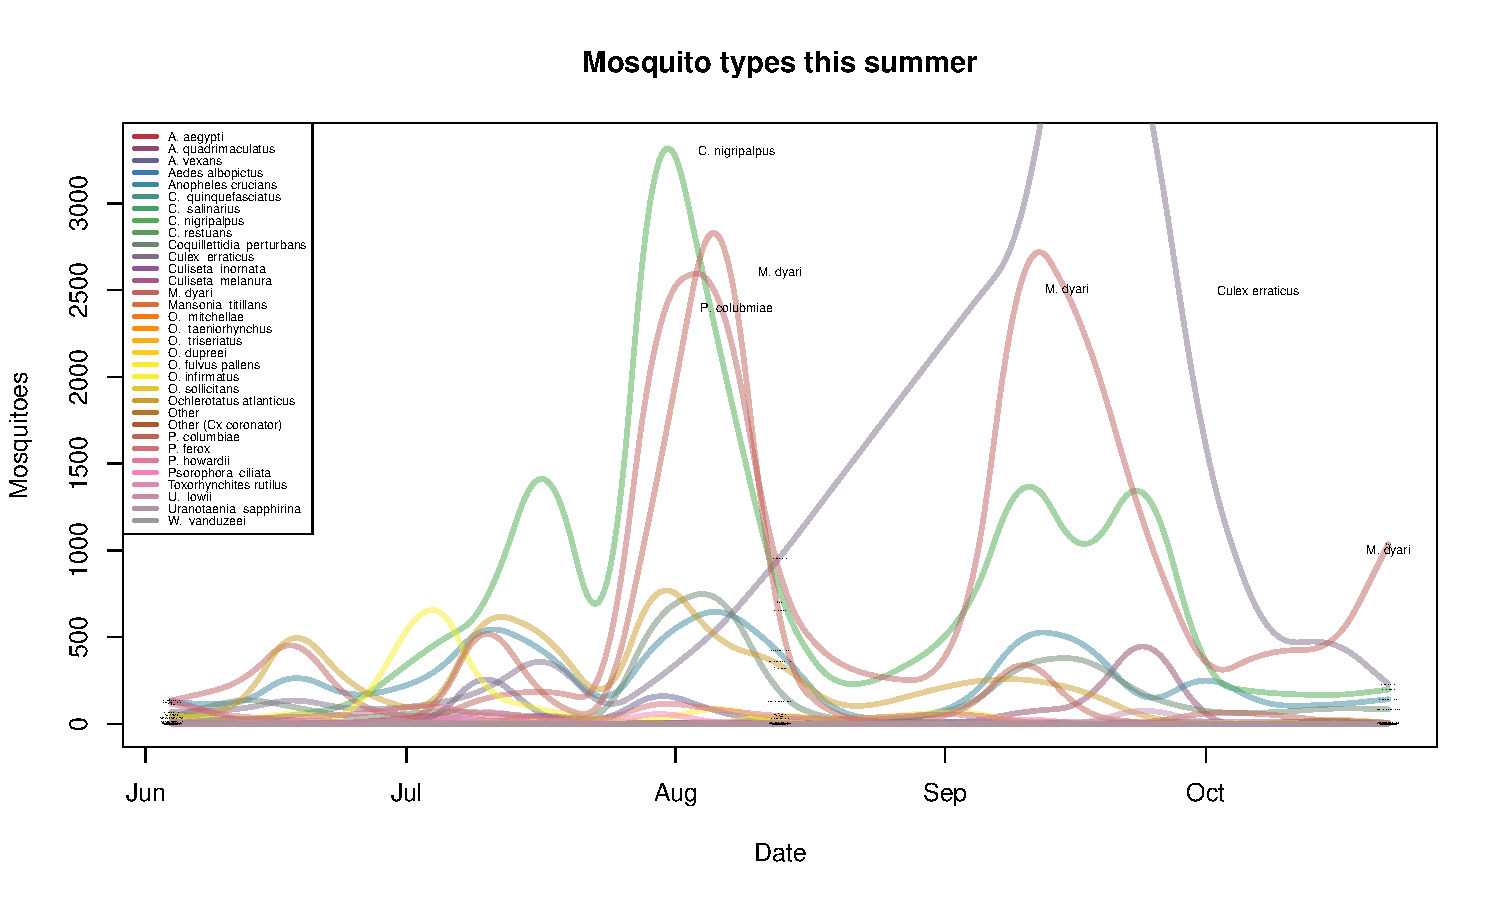
\includegraphics{mosq29octtype-002}
\subsection*{Breakdown by species of interest and date}
M. Dyari (a non-vector) is the most prevalent recent species.  Culex erraticus (a vector of multiple diseases, including WNV) accounted for much of the September spike (and was likely the culprit for the infection of our local case).  P. columbiae (non-vector) and C. nigripalpus (vector of equine encephalitii and WNV) accounted for the early August spike.

\begin{small}

\begin{table}[ht]
\centering
\begin{tabular}{rlrrrrr}
  \hline
 & date & Aedes albopictus & C. nigripalpus & Culex  erraticus & M. dyari & P. columbiae \\ 
  \hline
1 & 2013-06-04 & 0.00 & 57.00 & 69.00 & 135.00 & 1.00 \\ 
  2 & 2013-06-12 & 0.00 & 18.00 & 82.00 & 227.00 & 37.00 \\ 
  3 & 2013-06-18 & 3.00 & 49.00 & 149.00 & 530.00 & 19.00 \\ 
  4 & 2013-06-25 & 5.00 & 107.00 & 76.00 & 87.00 & 10.00 \\ 
  5 & 2013-07-04 & 4.00 & 455.00 & 108.00 & 27.00 & 27.00 \\ 
  6 & 2013-07-10 & 6.00 & 621.00 & 187.00 & 155.00 & 638.00 \\ 
  7 & 2013-07-17 & 5.00 & 1670.00 & 418.00 & 198.00 & 123.00 \\ 
  8 & 2013-07-24 & 1.00 & 254.00 & 60.00 & 117.00 & 8.00 \\ 
  9 & 2013-07-30 & 3.00 & 3801.00 & 260.00 & 2513.00 & 1424.00 \\ 
  10 & 2013-08-06 & 5.00 & 2157.00 & 547.00 & 2656.00 & 3330.00 \\ 
  11 & 2013-08-13 & 1.00 & 656.00 & 957.00 & 701.00 & 318.00 \\ 
  12 & 2013-08-20 & 4.00 & 136.00 & 1423.00 & 292.00 & 2.00 \\ 
  13 & 2013-09-03 & 15.00 & 512.00 & 2343.00 & 218.00 & 31.00 \\ 
  14 & 2013-09-10 & 7.00 & 1536.00 & 2781.00 & 2942.00 & 421.00 \\ 
  15 & 2013-09-17 & 2.00 & 902.00 & 5090.00 & 2313.00 & 48.00 \\ 
  16 & 2013-09-24 & 2.00 & 1526.00 & 3792.00 & 1094.00 & 0.00 \\ 
  17 & 2013-10-01 & 0.00 & 227.00 & 1462.00 & 249.00 & 68.00 \\ 
  18 & 2013-10-08 & 1.00 & 176.00 & 455.00 & 422.00 & 58.00 \\ 
  19 & 2013-10-16 & 1.00 & 162.00 & 487.00 & 430.00 & 11.00 \\ 
  20 & 2013-10-22 & 1.00 & 197.00 & 229.00 & 1036.00 & 0.00 \\ 
   \hline
\end{tabular}
\end{table}


\end{small}


\end{center}
The complete list of all 34 mosquito species is in the document named "mosquitospecies.xsl" (attached to this email).
\end{document}
